\documentclass[a4paper]{article}

\usepackage[english]{babel}
\usepackage[utf8]{inputenc}
\usepackage{amsmath}
\usepackage{hyperref}
\usepackage{subcaption}
\usepackage{graphicx}
\usepackage[colorinlistoftodos]{todonotes}

\title{Q10. Numerical Integration: (Dr. Beerli )\\Spring 2014}


\author{Amirhessam Tahmassebi}

\date{\today}

\begin{document}
\maketitle

Calculate this Integral
$$ I = \frac{1}{2\pi}\int_{-1}^{1}\int_{-1}^{1} e^{-(x^2+y^2)}dxdy$$ 

\section*{Method}
First of all, for more convenience, I tried to make the integral more easier in 1D due to the Symmetry of the problem. We have: \\

$$ I = [\frac{1}{\sqrt{2 \pi }}\int_{-1}^{1} e^{-(x^2)}dx]^2$$ 

\subsection*{Gauss Quadrature}
For this part, I have used John's Burkardt Gauss-Kronrod Package. It has both Gauss Rule and Gauss-Kronrod Weights and abscissas.

\subsection*{Clenshaw-Curtis Quadrature}


$$ I = \int_{-1}^{1} f(x) dx = \int_{0}^{\pi}f(cos\theta)sin\theta d\theta$$ 
We can say: \\
$$f(cos\theta) = \frac{a_0}{2} + \sum_{k=1}^{\infty} a_kcos(k\theta)$$
So, we will have: \\
$$ I = \int_{-1}^{1} f(x) dx = \int_{0}^{\pi}f(cos\theta)sin\theta d\theta = a_0 +\sum_{k=1}^{\infty} \frac{2a_{2k}}{1-(2k)^2} $$ 
With : \\
$$a_k = \frac{2}{\pi} \int_{0}^{\pi} f(cos\theta)cos(k\theta)d\theta$$


\subsection*{Romberg}
$$ I = I_{2n} + \frac{I_{2n}-I_{n}}{3}$$
Which I used trapezoidal rule for calculating each part of the fractions.

\subsection*{MonteCarlo}

For this part, we just need to produce N sample darts between our intervals which is -1 and 1. I have used uniform distribution. Then we find the value of each sample dart at our function, multiply with the length of our interval which is 2.

\section*{Results}

\subsection*{Gauss Quadrature}

The Integral Using Gauss rule :: I = 0.355072003479 \\
The Integral Using Gauss-Kronrod (N=6) :: I = 0.355072313218 \\
Relative Error of Integrals  = 4.36163263248e-07 \\



\begin{figure}[h]
\begin{subfigure}[b]{0.49\textwidth}
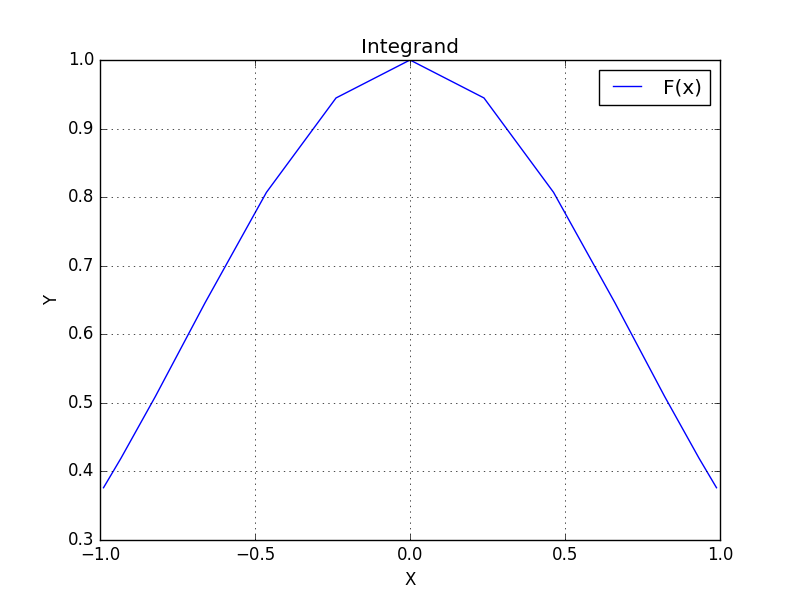
\includegraphics[width=\textwidth]{g1.png}
\caption{Integrand using Gauss Rule}
\end{subfigure}
\begin{subfigure}[b]{0.49\textwidth}
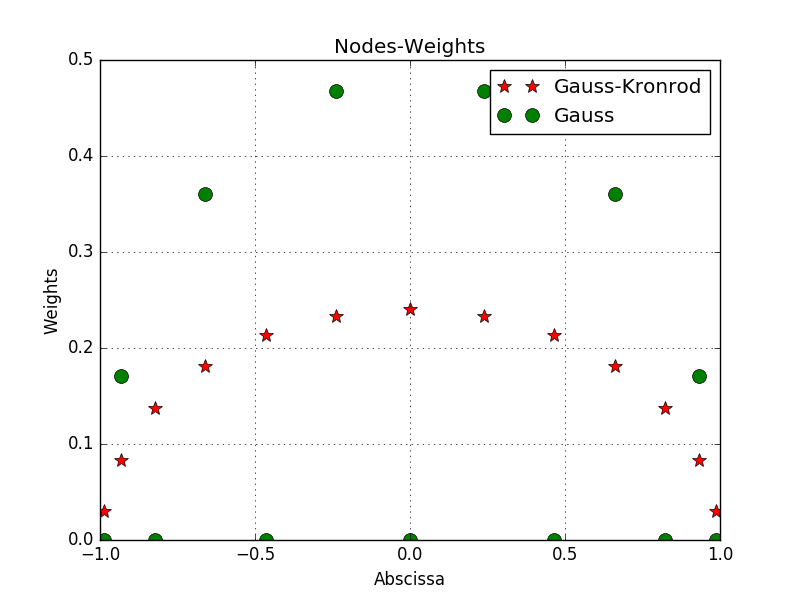
\includegraphics[width=\textwidth]{g2.png}
\caption{Gauss and Gauss-Kronrod Rule}
\end{subfigure}
\end{figure}

\subsection*{Clenshaw-Curtis Quadrature}
The Result using ClenShaw-Curtis Integration = 0.355072313219 \\

\subsection*{Romberg's Method}
Step = 1 , Romberg = 0.153168208369 , Norm = 0.201901791631\\
Step = 2 , Romberg = 0.445237854316 , Norm = 0.0901678543157\\
Step = 4 , Romberg = 0.35747361225 , Norm = 0.00240361224977\\
Step = 8 , Romberg = 0.355280298733 , Norm = 0.000210298733121\\
Step = 16 , Romberg = 0.355094403579 , Norm = 2.44035792558e-05\\
Step = 32 , Romberg = 0.355074869388 , Norm = 4.86938789629e-06 \\


\begin{center}

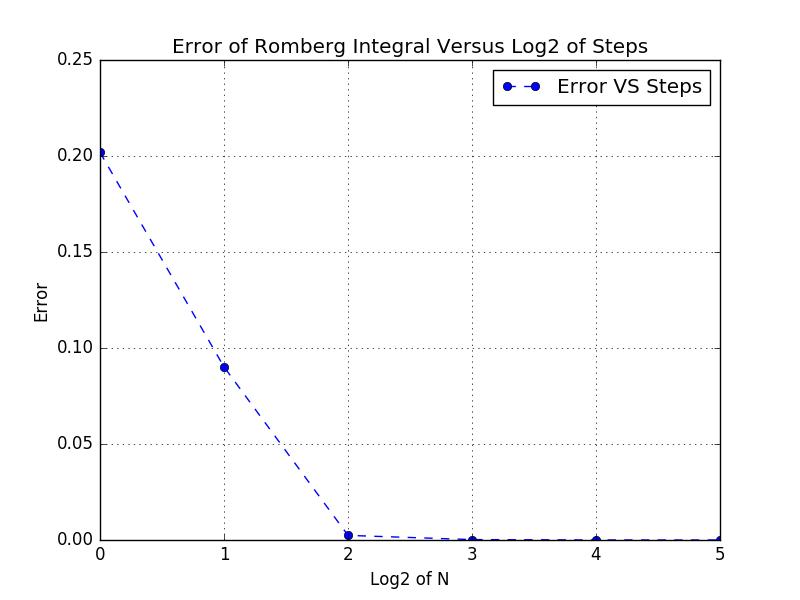
\includegraphics[width=\textwidth]{r1.png}

\end{center}

\subsection*{MonteCarlo}

The Result with 100000 darts = 0.355103269763 \\
Standard Deviation = 0.00632455532034 \\

\begin{center}

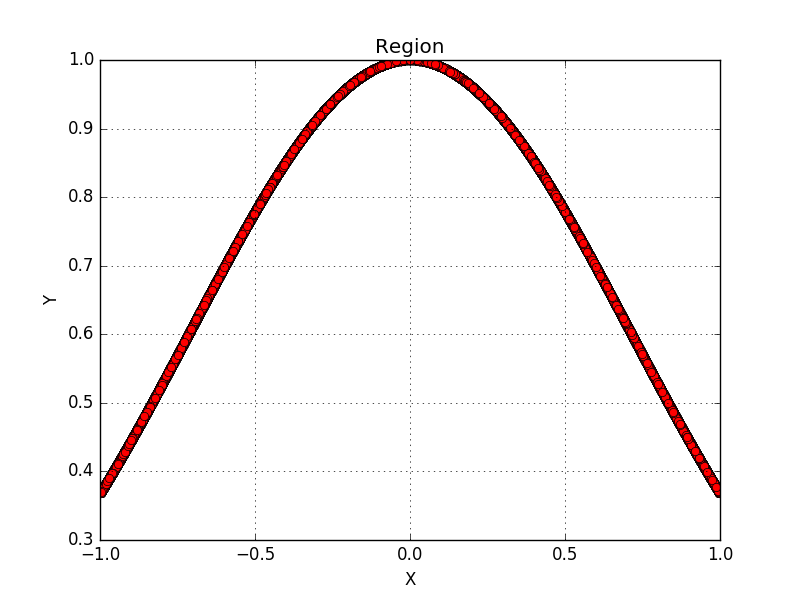
\includegraphics[width=\textwidth]{m1.png}

\end{center}












\end{document}